%%% -*- coding: utf-8 -*-
\newpage

\chapter{Learning}
\label{chap:learning}

\section{Deep Learning}
\label{sec:deep-learning}

Deep Learning is a branch of machine learning responsible for studying complex architectures, with the pourpose of learning patterns in data representations. The \textit{deep} in the name refers to the depth of layers in the architectures, as it can be very deep.

Most of the models in Deep Learning are composed of Artificial Neural Networks. Those neural networks were first proposed by McCulloch and Pitts~\cite{McCulloch1943}, in 1943, and were inspired by the processing and communication patterns in biological nervous systems, although there are many differences and even more from human brains. Those differences make the study of Artificial Neural Networks incompatible with the study of neuroscience.

\subsection{The perceptron}
The first ANN model was implemented by Frank Rosenblatt~\cite{Rosenblatt1958}, and was called \textit{the perceptron}. The perceptron was composed of multiple inputs, an output, a collection of weights and an activation function. It was capable of learning binary classification by supervised learning.

\begin{center}
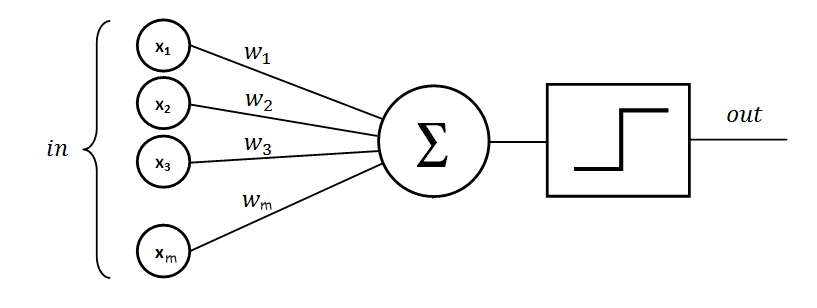
\includegraphics[width=1\columnwidth]{perceptron}
\end{center}

Mathmatically, the perceptron is a function that maps the input $\boldsymbol{x}$ to a binary output $\boldsymbol{f(x)}$.

\begin{minipage}{\textwidth}
\begin{center}
$
f(x)=\begin{cases}
1 & \text{ if } \boldsymbol{w \cdot x} + b > 0 \\
0 & \text{ otherwise }
\end{cases}
$
\end{center}

\vspace{0.5cm}

\hspace{4.5cm}$\boldsymbol{w \cdot x}$ is the dot product $\sum_{i=1}^{m}w_{i}x_{i}$,

\hspace{4.5cm}$w$ is a vector of weights

\hspace{4.5cm}$m$ is the number of inputs

\hspace{4.5cm}$b$ is the bias
\end{minipage}

\vspace{0.5cm}

This model was heavily criticized because it couldn't learn a simple XOR function, as it can only simulate linearly separable functions. To overcome this, Rumelhart, Hinton and Willians~\cite{Rumelhart1986} proposed the Backpropagation algorithm, which implemented another layer and finally was capable of simulating non-linearity.

Nowadays, Artificial Neural Networks are composed of multiple neurons, and multiple layers of neurons. Each neuron works similar to a perceptron.

\subsection{Activation Functions}

As the name sugests, the activation functions are responsible for setting the activation of a neuron, in other words, it sets how the input signal is passed to the output.

The first activation function, proposed by McCulloch and Pitts, was the threshold fuction. This function is binary, it is equals to 1 (passes the signal) if the input signal is greater than 0, and it does not passes the signal otherwise, as in above perceptron description.

Another common activation function is the sigmoid. Unlike the threshold function, the sigmoid function is smoother, and can be mathmatically described as $\phi(x) = 1/(1+e^{-x})$. This function is usually used in the last layer of classification models to describe the probability of the signal being 0 or 1, and that's where the smoothness is helpfull instead of the binary threshold.

Then, there is the rectifier function $\phi(x) = max(0, x)$. Nowadays, it is one of the most popular functions for Artificial Neural Networks, thanks to the work of Glorot, Bordes and Bengio, who proved it allowed faster and better training of ANNs~\cite{Glorot2010}.

Finally, there is the hyperbolic tangent function, which is similar to the sigmoid function, but it goes from 1 to -1. The sigmoid function can "stuck" the training of ANNs, because when a strongly-negative input is provided, the sigmoid function outputs values very near to zero, inactivating the neuron instead of passing a negative signal~\cite{Glorot2010.2}. Thus, the hyperbolic tangent function is usually preferable. Mathmatically, it can be described as $\phi(x) = (1-e^{-2x})/(1+e^{-2x})$.

\vspace{0.5cm}

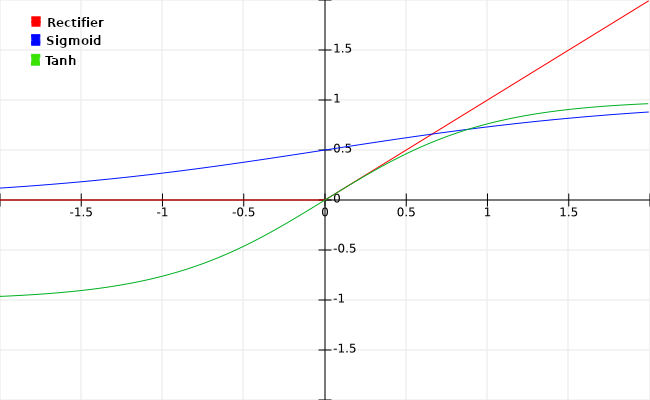
\includegraphics[width=1\columnwidth]{activation-functions}



\section{Reinforcement Learning}
\label{sec:reinforcement-learning}

%%% Local Variables:
%%% mode: latex
%%% TeX-master: thesis.tex
%%% End:
